\chapter{Lezione 9}
\label{chap:lezione_09}

\begin{flushright}
\textit{Data: 23/10/2025}
\end{flushright}


\section{Generalizzazione del Criterio di Harris}

Riprendiamo la discussione sul Criterio di Harris iniziata nella lezione precedente. Stiamo analizzando la stabilità del punto fisso di un sistema puro rispetto all'introduzione di disordine (diluizione), modellizzato come fluttuazioni locali della temperatura critica $T_c(\vec{x})$. Definiamo la temperatura ridotta locale $t(\vec{x})$, che misura la distanza dalla criticità in un punto $\vec{x}$:
\begin{equation}
t(\vec{x}) \propto T - T_c(\vec{x})
\end{equation}

\noindent Assumiamo che le fluttuazioni del disordine siano correlate spazialmente. La funzione di correlazione connessa del campo di temperatura ridotta è data da:
\begin{equation}
\overline{t(\vec{x})t(\vec{y})}^c \propto |\vec{x}-\vec{y}|^{-a}
\end{equation}
dove l'esponente $a$ caratterizza il raggio delle correlazioni del disordine.
Consideriamo un volume di correlazione $V \sim \xi^D$. La media spaziale della temperatura ridotta su questo volume è:
\begin{equation}
t_V = \frac{1}{V} \int_V d^D \vec{x} \, t(\vec{x})
\end{equation}
Il valore medio atteso di questa quantità è semplicemente la temperatura ridotta macroscopica del sistema, $t = \overline{t_V}$. Tuttavia, a causa del disordine, ogni regione avrà un valore leggermente diverso. Ci interessa calcolare la varianza di queste fluttuazioni su scala $\xi$:

\begin{equation}
\Delta^2 = \overline{t_V^2} - t^2
\end{equation}

\noindent Dall'analisi dell'integrale della funzione di correlazione sul volume $V$, otteniamo tre comportamenti distinti per la fluttuazione $\Delta$ in funzione della lunghezza di correlazione $\xi$, a seconda del rapporto tra l'esponente di decadimento $a$ e la dimensione spaziale $D$:

\begin{equation}
\Delta^2 = \overline{t_V^2} - t^2 \propto 
\begin{cases} 
\xi^{-D} & a > D \quad \text{(Disordine a corto raggio/uncorrelated)} \\
\xi^{-D} \log \xi & a = D \quad \text{(Caso marginale)} \\
\xi^{-a} & a < D \quad \text{(Disordine a lungo raggio/correlated)}
\end{cases}
\end{equation}

\subsection{Analisi della Stabilità}

Per determinare se il disordine è rilevante, dobbiamo confrontare l'ampiezza delle fluttuazioni del disordine ($\Delta$) con la distanza media dal punto critico ($t$). Avvicinandosi alla transizione ($\xi \to \infty, t \to 0$), il disordine è irrilevante se le fluttuazioni diventano trascurabili rispetto alla media, ovvero se il rapporto $\Delta^2 / t^2$ tende a zero.

\noindent Ricordando la relazione di scaling $\xi \sim t^{-\nu}$, analizziamo il rapporto $\Delta^2 / t^2$:

\begin{equation}
\frac{\Delta^2}{t^2} \propto \begin{cases} 
t^{\nu D - 2} & , a > D \\
t^{\nu D - 2} \log t & , a = D \\
t^{\nu a - 2} & , a < D
\end{cases}
\end{equation}

Possiamo riscrivere gli esponenti usando la relazione di iperscaling $\alpha = 2 - D\nu$:
\begin{itemize}
    \item Caso $a > D$ \textbf{(Harris Standard):} L'esponente diventa $\frac{2 - D\nu}{\nu} = \frac{\alpha}{\nu}$.
    Il disordine è \textbf{irrilevante} se $\Delta^2/t^2 \to 0$, ovvero se l'esponente è negativo. Questo implica $\alpha < 0$.
    \item Caso $a < D$ \textbf{(Weinrib-Halperin):} L'esponente è $\frac{2}{\nu} - a$. La condizione di stabilità richiede $a > 2/\nu$, ovvero $a\nu > 2$.
\end{itemize}

\begin{tcolorbox}[colback=colorD!10, colframe=colorD!60!colorE, , coltitle=white, title=\textbf{Conclusione sulla Rilevanza}]
Il disordine è \textbf{irrilevante} se il calore specifico del sistema puro non diverge (o diverge debolmente).
\begin{itemize}
    \item Se $\alpha < 0$, il disordine è \textbf{irrilevante}. Il sistema mantiene gli esponenti critici del caso puro.
    \item Se $\alpha > 0$, il disordine è \textbf{rilevante}. Il punto fisso puro è instabile.
\end{itemize}
\end{tcolorbox}

\subsubsection{Casi Fisici Notevoli}

Analizziamo alcuni casi specifici del modello di Ising:
\begin{itemize}
    \item \textbf{Ising 2D:} Sappiamo che $\alpha = 0$ (divergenza logaritmica, $\alpha_{2D} = 0_{\log}$). Questo è un caso marginale.
    \item \textbf{Ising 3D:} Si ha $\alpha > 0$ ($\alpha \approx 0.11$). In tre dimensioni, il punto fisso puro è instabile rispetto all'introduzione di disordine (anche a corto raggio).
\end{itemize}

\noindent La Figura \ref{fig:fixed_points} mostra come (nel caso 3D) il punto fisso puro, situato sull'asse delle temperature ($p=0$), sia instabile a causa della rilevanza del disordine ($\alpha > 0$). Le traiettorie del flusso RG si allontanano da esso. Tuttavia, non si dirigono verso il punto fisso di percolazione a $T=0$ (che è a sua volta instabile lungo la linea critica), ma convergono verso un nuovo punto fisso stabile situato a temperatura finita, detto \textbf{Random Fixed Point}. Questo punto fisso controlla il comportamento critico lungo l'intera linea di transizione di fase per $p > 0$, imponendo una nuova classe di universalità caratterizzata da esponenti critici diversi sia da quelli del modello puro che da quelli della percolazione.

\begin{figure}[h]
    \centering
    \begin{tikzpicture}[
        >=Stealth,          % Stile della punta delle frecce
        font=\sffamily,     % Font sans-serif
        scale=1.3,          % Scala generale
        thick               % Linee leggermente più spesse
    ]

    % --- Definizioni Variabili ---
    \def\xmax{6}
    \def\ymax{5}
    \def\pc{1.8}
    \def\bone{5.5}
    \def\Tc{4.2}

    % --- Definizioni Stili ---
    \tikzset{
        flow_arrows/.style={
            decoration={
                markings,
                % Frecce prima del punto centrale (puntano avanti)
                mark=at position 0.15 with {\arrow[scale=1.5, red!80!black]{>}},
                mark=at position 0.35 with {\arrow[scale=1.5, red!80!black]{>}},
                % Frecce dopo il punto centrale (puntano indietro, verso il centro)
                mark=at position 0.65 with {\arrow[scale=1.5, red!80!black]{<}},
                mark=at position 0.85 with {\arrow[scale=1.5, red!80!black]{<}}
            },
            postaction={decorate}
        },
        % Stile comune per i punti fissi (cerchio bianco con bordo rosso scuro)
        fixed_point/.style={
            fill=white, 
            draw=red!80!black, 
            line width=1.5pt,
            circle,
            inner sep=0pt,
            minimum size=6pt
        }
    }

    % --- 1. Linee di proiezione (Grigie tratteggiate) ---
    \draw[dashed, gray!80, line width=0.8pt] (0, \Tc) -- (\bone, \Tc) -- (\bone, 0);

    % --- 2. La Curva Critica (Blu Moderno) ---
    \draw[cyan!30!blue, line width=1.8pt, flow_arrows] 
        (\pc, 0) to[out=85, in=180] coordinate[pos=0.5] (CenterPoint) (\bone, \Tc);

    % --- 3. Punti Fissi e Etichette ---
    
    % A) Punto Iniziale (pc) - Instabile
    \node[fixed_point] at (\pc, 0) {};
    \node[red!80!black, font=\footnotesize, align=left] at (\pc+0.9, 0.3) {\textbf{Unstable}};

    % B) Punto Centrale - Stabile
    \node[fixed_point] at (CenterPoint) {};
    % Etichetta per il punto centrale (spostata in alto a sinistra per chiarezza)
    \node[above left=2pt, font=\small, align=right] at (CenterPoint) 
        {\textbf{RFP}\\\textbf{Stable}};

    % C) Punto Finale (1) - Instabile
    \node[fixed_point] at (\bone, \Tc) {};
    \node[red!80!black, font=\footnotesize, above=5pt] at (\bone, \Tc) {\textbf{Unstable}};

    % --- 4. Assi Cartesiani ---
    \draw[->, line width=1.2pt] (0,0) -- (\xmax + 0.3, 0) node[right] {$p$};
    \draw[->, line width=1.2pt] (0,0) -- (0, \ymax + 0.3) node[above] {$T$};

    % --- 5. Etichette Assi ---
    \node[left] at (0, \Tc) {$T_c(1)$};
    \node[below] at (\pc, 0) {$p_c$};
    \node[below] at (\bone, 0) {$1$};

    \end{tikzpicture}
    \caption{Diagramma schematico dei punti fissi nel piano $(p, T)$. La curva rappresenta la linea critica. Il punto fisso stabile (Random Fixed Point) si trova lungo la curva, intermedio tra i due punti fissi instabili del modello puro ($p=1$) e della percolazione ($p_c$).}
    \label{fig:fixed_points}
\end{figure}





\newpage

\section{Fase di Griffiths e Zeri di Lee-Yang}

Consideriamo la regione del diagramma di fase sotto la temperatura critica del modello puro ($T < T_c^{pure}$), ma sopra la temperatura critica del sistema diluito ($T > T_c(p)$). Questa regione è chiamata \textbf{Fase di Griffiths}.
In questa fase non c'è ordine magnetico a lungo raggio ($m=0$), ma la dinamica e le proprietà analitiche sono peculiari.

\begin{figure}[H]
    \centering
    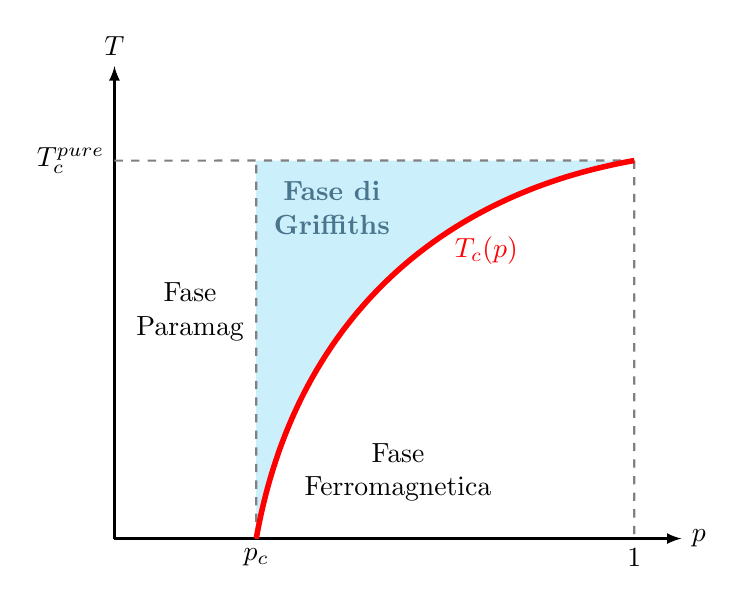
\begin{tikzpicture}[scale=1.2, >=latex]
        % Assi
        \draw[->, thick] (0,0) -- (6,0) node[right] {$p$};
        \draw[->, thick] (0,0) -- (0,5) node[above] {$T$};

        % Coordinate
        \coordinate (Pc) at (1.5, 0);       % Soglia di percolazione
        \coordinate (Pure) at (5.5, 4);     % Punto puro (p=1, Tc_pure)
        \coordinate (Zero) at (0,0);

        % Definizione area Fase di Griffiths (Senza pattern problematici)
        % Riempiamo l'area compresa tra la curva critica T_c(p) e la retta T_c_pure
        % Usiamo 'opacity' per evitare blocchi neri e vedere le linee sotto
        \fill[cyan, opacity=0.2] (Pc) to[out=80, in=190] (Pure) -- (1.5, 4) -- cycle;

        % Linee guida e curve (disegnate SOPRA il riempimento)
        
        % Linea T_c pure (orizzontale tratteggiata)
        \draw[dashed, thick, gray] (0, 4) node[left, black] {$T_c^{pure}$} -- (Pure);
        \draw[dashed, thick, gray] (Pure) -- (5.5, 0) node[below, black] {$1$};
        \draw[dashed, thick, gray] (Pc) node[below, black] {$p_c$} -- (1.5, 4); % Linea verticale pc per chiudere la regione

        % Curva critica T_c(p)
        \draw[line width=2pt, red] (Pc) to[out=80, in=190] (Pure);
        \node[red, below right] at (3.5, 3.3) {$T_c(p)$};

        % Etichette Fasi
        \node[align=center, font=\bfseries, color=cyan!50!black] at (2.3, 3.5) {Fase di\\Griffiths};
        \node[align=center, color=black] at (3, 0.7) {Fase\\Ferromagnetica};
        \node[align=center, color=black] at (0.8, 2.4) {Fase\\Paramag};

    \end{tikzpicture}
    \caption{Diagramma di fase schematico. La Fase di Griffiths in azzurro è la regione in cui la temperatura è inferiore alla temperatura critica del sistema puro ($T < T_c^{pure}$) ma superiore alla temperatura critica effettiva del sistema diluito ($T > T_c(p)$). Qui il sistema è globalmente paramagnetico ma contiene cluster localmente ordinati.}
    \label{fig:griffiths_phase_fixed}
\end{figure}

\subsection{Zeri di Lee-Yang}

Per comprendere la natura matematica delle transizioni di fase, Lee e Yang proposero di analizzare gli zeri della funzione di partizione nel piano complesso.
Consideriamo il modello di Ising con $N$ spin. L'Hamiltoniana generica è:
\begin{equation}
H(\vec{S}) = - J \sum S_i S_j - h \sum S_i
\end{equation}

\noindent La funzione di partizione è $\mathcal{Z} = \sum_{\vec{S}} e^{-\beta H(\vec{S})}$.
Definendo le variabili $X = \exp(-2\beta J)$ e $z = \exp(-2\beta h)$ (\textbf{fugacità}), possiamo riscrivere il termine di campo:
\begin{equation}
e^{-\beta h S_i} = e^{\beta h} \begin{cases} 1 & \text{se } S_i = -1 \\ y & \text{se } S_i = +1 \end{cases}
\end{equation}
$\mathcal{Z}$ diventa un polinomio in $X$ di grado pari al numero di interazioni e in $z$ di grado $N$.

\hfill 

\noindent Secondo il teorema di Lee-Yang, gli zeri di $\mathcal{Z}$ nel piano complesso della fugacità $z$:
\begin{enumerate}
    \item Non hanno zeri sull'asse reale ($Re \, z$).
    \item Giacciono tutti sul cerchio unitario ($|z|=1$), che corrisponde a un campo magnetico puramente immaginario ($h$ immaginario puro).
\end{enumerate}


\begin{tcolorbox}[colback=yellow!25, colframe=yellow!75!orange, coltitle=black, title=\textbf{Teorema del Cerchio (Lee-Yang)}]
Per il modello di Ising ferromagnetico, tutti gli zeri della funzione di partizione giacciono sul cerchio unitario nel piano complesso della fugacità:
\begin{equation}
|z| = 1 \implies \text{Re}(h) = 0, \quad \text{Im}(h) \neq 0 \implies h \; \text{immaginario puro}
\end{equation}
\end{tcolorbox}


\begin{figure}[h]
    \centering
    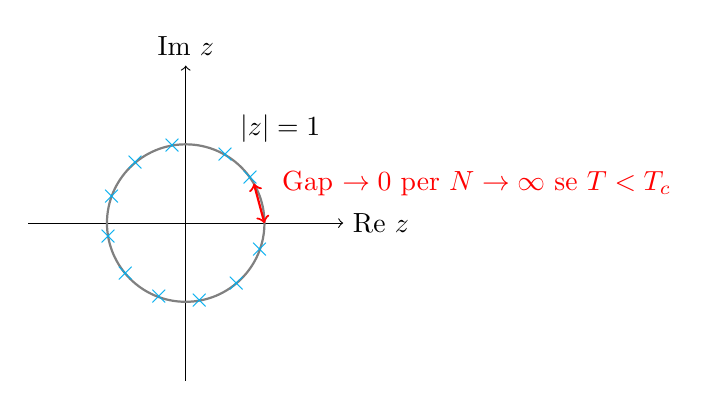
\begin{tikzpicture}[scale=1.]
        % Assi
        \draw[->] (-2,0) -- (2,0) node[right] {Re $z$};
        \draw[->] (0,-2) -- (0,2) node[above] {Im $z$};
        
        % Cerchio unitario
        \draw[thick, gray] (0,0) circle (1);
        \node at (1.2, 1.2) {$|z|=1$};

        % Zeri (croci)
        \foreach \angle in { 35, 60, 100, 130, 160, 190, 220, 250, 280, 310, 340}
            \node at (\angle:1) {\textcolor{cyan}{$\mathbf{\times}$}};
            
        % Gap
        \draw[<->, red, thick] (1,0) -- (30:1);
        \node[red, right] at (1.1, 0.5) {Gap $\to 0$ per $N \to \infty$ se $T < T_c$};
        
    \end{tikzpicture}
    \caption{Distribuzione degli zeri di Lee-Yang nel piano complesso della fugacità $z$. Nel limite termodinamico e per $T < T_c$, gli zeri si addensano verso il punto $z=1$ (asse reale positivo), "pizzicando" l'asse reale e impedendo il prolungamento analitico.}
    \label{fig:lee_yang}
\end{figure}

\noindent Per un sistema finito, gli zeri non toccano mai l'asse reale positivo ($z=1 \iff h=0$), quindi la funzione di partizione è analitica e non ci sono transizioni di fase.
Nel limite termodinamico ($N \to \infty$):
\begin{itemize}
    \item Se $T > T_c$: Gli zeri rimangono staccati dall'asse reale. Esiste un gap che permette lo sviluppo analitico in serie di $h$ attorno a $h=0$.
    \item Se $T < T_c$: Gli zeri si accumulano e "pizzicano" l'asse reale in $z=1$. Questo crea una barriera di non-analiticità che separa la fase $h>0$ da quella $h<0$, impedendo la continuazione analitica e generando la \textbf{discontinuità} tipica della transizione del primo ordine (rottura spontanea di simmetria).
\end{itemize}

\subsection{Singolarità di Griffiths}

Per comprendere la natura matematica della Fase di Griffiths, analizziamo come si comporta la magnetizzazione del sistema decomponendolo in cluster indipendenti.
Nella fase paramagnetica (o di Griffiths), possiamo immaginare il sistema composto da cluster finiti $c$ di spin connessi.
Sia $P_{\lambda, c}$ la probabilità di trovare un cluster $c$ all'interno di un volume macroscopico $\lambda$.
La densità di magnetizzazione del sistema nel volume $\lambda$ è la media pesata delle magnetizzazioni dei singoli cluster:

\begin{equation}
m_{\lambda} = \frac{1}{|\lambda|} \sum_{c} P_{\lambda,c} |c| m_c
\end{equation}

\noindent Per ogni cluster finito $c$, possiamo scrivere la funzione di partizione $\mathcal{Z}_c$ utilizzando il teorema di Lee-Yang. Introdotta la variabile fugacità $y = e^{-2\beta h}$, $\mathcal{Z}_c$ è un polinomio in $y$ di grado $|c|$ (numero di spin nel cluster):

\begin{equation}
\mathcal{Z}_c(y) \propto y^{-|c|/2} \prod_{a=1}^{|c|} (y - \zeta_a(c))
\end{equation}

\noindent dove $\zeta_a(c)$ sono gli zeri della funzione di partizione del cluster $c$, che giacciono tutti sul cerchio unitario nel piano complesso ($|\zeta_a| = 1$).

\noindent L'energia libera per spin del cluster $c$ è data da:
\begin{equation}
f_c = -\frac{1}{\beta |c|} \log \mathcal{Z}_c = \frac{\log \mathcal{Z}_c}{2\beta} - \frac{1}{\beta |c|} \sum_{a=1}^{|c|} \log(y - \zeta_a(c))
\end{equation}

\noindent La magnetizzazione del singolo cluster $m_c$ si ottiene derivando l'energia libera rispetto al campo (o equivalentemente rispetto a $y$):
\begin{equation}
m_c = - \frac{\partial f_c}{\partial h} = -1 + \frac{2y}{|c|} \sum_{a=1}^{|c|} \frac{1}{y - \zeta_a(c)}
\end{equation}

\noindent Sostituendo questa espressione nella formula della magnetizzazione totale $m_{\lambda}$:

\begin{equation}
m_{\lambda} = -p + \frac{2y}{|\lambda|} \sum_{c} P_{\lambda,c} \sum_{a=1}^{|c|} \frac{1}{y - \zeta_a(c)}
\end{equation}

\noindent A questo punto, notiamo che cluster diversi possono avere zeri nella stessa posizione. Possiamo raggruppare i termini sommando sugli $N_A$ zeri \textit{distinti} possibili nel sistema. Definiamo un "peso" o densità spettrale degli zeri $\eta_a(\lambda)$:

\begin{equation}
m_{\lambda} = -p + \frac{2y}{|\lambda|} \sum_{a=1}^{N_A} \frac{\eta_a(\lambda)}{y - \zeta_a}
\end{equation}

\noindent dove il coefficiente $\eta_a(\lambda)$ raccoglie i contributi di tutti i cluster che possiedono uno zero in posizione $\zeta_a$, pesati dalla loro probabilità di occorrenza e dalla molteplicità $\mu_a(c)$ dello zero nel cluster:

\begin{equation}
\eta_a(\lambda) = \frac{1}{|\lambda|} \sum_{c \, :\, \zeta_a(c) = \zeta_a} \mu_a(c) P_{c,\lambda} > 0
\end{equation}

\noindent Vale inoltre la regola di somma (poiché la somma delle probabilità deve essere normalizzata rispetto alla densità dei siti attivi):
\begin{equation}
p = \sum_a \eta_a(\lambda)
\end{equation}

\subsubsection*{Analisi della Singolarità}

L'espressione finale per $m_{\lambda}$ mostra che \textbf{la magnetizzazione è una somma di poli nel piano complesso.}
\begin{itemize}
    \item Se $|y| \neq 1$, la funzione è analitica (somma di termini regolari).
    \item I problemi sorgono quando gli zeri si avvicinano all'asse reale positivo ($y \to 1$).
\end{itemize}

\noindent Consideriamo un cluster molto grande e compatto, di taglia $|c| \approx bN$. Questo cluster avrà zeri molto vicini all'asse reale (gap $\sim 1/N$). Tuttavia, la probabilità $P_{c,\lambda}$ di trovare un tale cluster "puro" in un sistema diluito è esponenzialmente piccola rispetto alla sua taglia:

\begin{equation}
P_{c,\lambda} \propto p^{|c|} = p^{bN} = e^{-d N}  \quad \quad \text{con } d = b \log(1/p)
\end{equation}

Di conseguenza, i poli che si avvicinano all'asse reale hanno un residuo $\eta_a$ che tende a zero esponenzialmente.
Questo rende la funzione $C^\infty$ (liscia) sull'asse reale, ma \textbf{non analitica}. Queste sono le \textbf{Singolarità di Griffiths}: punti di non analiticità dovuti a configurazioni rare ma inevitabili nel limite termodinamico.


\subsection{Dinamica dei Sistemi Disordinati}
L'effetto più evidente della Fase di Griffiths non è nella termodinamica statica, ma nella \textbf{dinamica}. Le regioni rare e dense (i cluster ferromagnetici locali) agiscono come trappole dinamiche, rallentando enormemente il rilassamento del sistema. Per studiare l'evoluzione temporale, introduciamo la \textbf{Dinamica di Glauber} (o equivalentemente un algoritmo Monte Carlo tipo Metropolis).

\noindent Consideriamo l'Hamiltoniana di Ising:
\begin{equation}
H(\vec{S}) = - \sum_{i,j} J_{ij} S_i S_j - \sum_i h_i S_i
\end{equation}

\noindent Definiamo il \textbf{campo locale} $b_i(t)$ che agisce sullo spin $i$-esimo al tempo $t$:
\begin{equation}
b_i(t) = \sum_{j} J_{ij} S_j(t) + h_i
\end{equation}

\noindent La regola di aggiornamento stocastico per lo spin $S_i$ al tempo $t+1$ è data dalle probabilità di transizione:
\begin{equation}
S_i(t+1) = \begin{cases} 
+1 & \text{con probabilità } \frac{1 + \tanh(\beta b_i(t))}{2} \\
-1 & \text{con probabilità } \frac{1 - \tanh(\beta b_i(t))}{2}
\end{cases}
\end{equation}

\noindent Il valore di aspettazione dello spin al passo successivo è quindi determinato interamente dal campo locale:
\begin{equation}
\langle S_i(t+1) \rangle = \tanh(\beta b_i(t))
\end{equation}

\subsubsection{Osservabili Dinamiche}

Per caratterizzare l'evoluzione del sistema verso l'equilibrio (o il suo mancato raggiungimento), monitoriamo due quantità principali.

\textbf{1. Autocorrelazione Temporale:}
Misura la memoria del sistema rispetto a una configurazione precedente (o quella iniziale):
\begin{equation}
C(t, t') = \frac{1}{N} \sum_i \langle S_i(t) S_i(t') \rangle
\end{equation}

\noindent Questa quantità ci dice "quanto il sistema ricorda la sua storia". È una variabile random che va mediata sulla dinamica di Glauber (realizzazioni del rumore termico).

\textbf{2. Correlazione Spaziale a tempi uguali:}
Misura la formazione di domini ordinati al tempo $t$:
\begin{equation}
G(r, t) = \frac{1}{N} \sum_{|i-j|=r} \langle S_i(t) S_j(t) \rangle
\end{equation}

\noindent Tipicamente ci aspettiamo un decadimento esponenziale che definisce la lunghezza di correlazione dinamica $\xi(t)$:
\begin{equation}
G(r, t) \propto e^{-r/\xi(t)}
\end{equation}

\noindent L'evoluzione temporale di $\xi(t)$ segue leggi di scala diverse a seconda della fase in cui ci troviamo. In un processo di ordinamento standard (coarsening), ci aspettiamo una crescita a legge di potenza:
\begin{equation}
\xi(t) \sim t^{1/2} \quad \text{(diffusiva)}
\end{equation}

\noindent A tempi lunghi, $\xi(t)$ satura al valore di equilibrio termodinamico $\xi_{eq}$ (se finito) o alla taglia del sistema $L$ (se siamo in fase critica o ordinata).
\begin{equation}
\xi(t) \to \xi_{eq} \implies G_{eq}(r) = \frac{1}{N_r} \sum_{|i-j|=r} \langle S_i S_j \rangle_{\text{Gibbs-Boltzmann}}
\end{equation}

\begin{figure}[H]
    \centering
       \begin{tikzpicture}[scale=1.2]
        % Assi
        \draw[->, thick] (0,0) -- (6,0) node[right] {$\ln(t)$};
        \draw[->, thick] (0,0) -- (0,4) node[above] {$\ln(\xi(t))$};
        
        % Crescita libera
        \draw[thick, violet] (0,0) -- (3, 2) node[midway, below right] {$\sim t^{1/2}$};
        
        % Saturazione Equilibrio
        \draw[thick, violet] (3,2) .. controls (4, 2.5) .. (6, 2.6);
        \node[right, violet] at (6, 2.6) {$\xi_{eq}(T)$};
        
        % Taglia Finita (System Size)
        \draw[dashed, teal, thick] (3,2) -- (4, 3);
        \draw[thick, teal] (4,3) -- (6, 3);
         \draw[dashed, magenta, thick] (4,3) -- (5, 4);
        \node[right, teal] at (6, 3) {Taglia $L$ (Effetti di taglia finita)};
        \node[right, magenta] at (5.1, 4) {Taglia infinita};


    \end{tikzpicture}
    \caption{Crescita della lunghezza di correlazione dinamica $\xi(t)$ in scala log-log. Inizialmente segue una legge di potenza (diffusiva, $\xi \sim t^{1/2}$). A tempi lunghi satura: o al valore di equilibrio termodinamico $\xi_{eq}$ (se siamo nella fase paramagnetica/Griffiths) o alla taglia del sistema $L$ (se siamo nella fase ordinata o critica).}
    \label{fig:dynamic_growth}
\end{figure}


Nella fase di Griffiths, la dinamica diventa estremamente lenta ("slow dynamics"). Sebbene $\xi_{eq}$ sia finita, il tempo per raggiungerla può essere enorme a causa delle barriere di energia libera introdotte dai cluster rari.

